% Chapter 1

\chapter{Introducción General} % Main chapter title

\label{Chapter1} % For referencing the chapter elsewhere, use \ref{Chapter1} 
\label{IntroGeneral}

%----------------------------------------------------------------------------------------

% Define some commands to keep the formatting separated from the content 
\newcommand{\keyword}[1]{\textbf{#1}}
\newcommand{\tabhead}[1]{\textbf{#1}}
\newcommand{\code}[1]{\texttt{#1}}
\newcommand{\file}[1]{\texttt{\bfseries#1}}
\newcommand{\option}[1]{\texttt{\itshape#1}}
\newcommand{\grados}{$^{\circ}$}

%----------------------------------------------------------------------------------------

%\section{Introducción}

%----------------------------------------------------------------------------------------
\section{Descripcion General del Trabajo}

El proyecto aquí presentado consiste en un sistema de adquisición portátil para medición de parámetros biomédicos en animales grandes. En este proyecto se tiene particular interés en la medición del parámetro biológico denominado \enquote{velocidad de onda de pulso (VOP)}, cuyo método de cálculo más aceptado consiste en el registro simultáneo de señales de presión intraarterial en dos puntos del árbol arterial. Conociendo la distancia y el desfasaje temporal entre estas mediciones de presión, se puede estimar la VOP como su cociente. Esto puede verse graficado en la figura \ref{fig:vop}.

\begin{figure}[!htbp]
	\centering
	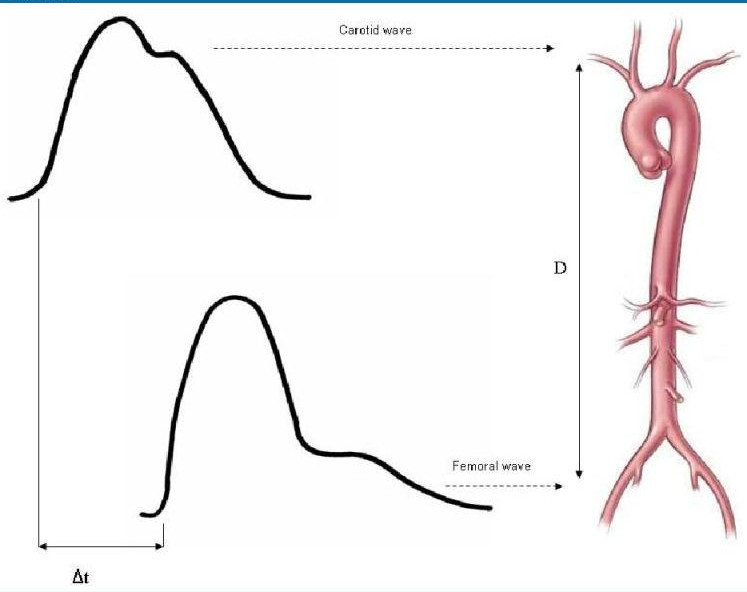
\includegraphics[width=\textwidth]{./Figures/VOP.jpg}
	\caption{Medición de VOP a partir de dos mediciones de la curva de presión, con un desfasaje temporal conocido}
	\label{fig:vop}
\end{figure}

El equipo consiste en un sistema embebido portátil basado en un microcontrolador ARM de 32 bits, Cortex M3: LPC1769, un conversor analógico digital de alta resolución (ADS1292), módulos de comunicación (serie, BLE, USB), almacenamiento masivo (SD) y módulo de regulación de energía y carga de batería. Puede verse un diagrama en bloques en la Figura \ref{fig:diag_bloques} . Para este proyecto se utilizaron en forma intensiva la gran mayoría de los contenidos y herramientas vistas durante el Curso de Especialización CESE. Se utilizaron técnicas de Gestión de Proyectos, documentación manual y automática del trabajo, sistema de versionado de software y hardware. En cuanto a lo técnico se emplearon conocimientos específicos sobre arquitectura del microcontrolador, modelos de programación, sistema operativo de tiempo real freeRTOS, protocolos de comunicación (BLE, SPI, USB, y de alto nivel), testing unitarios, etc.


\begin{figure}[!htbp]
	\centering
	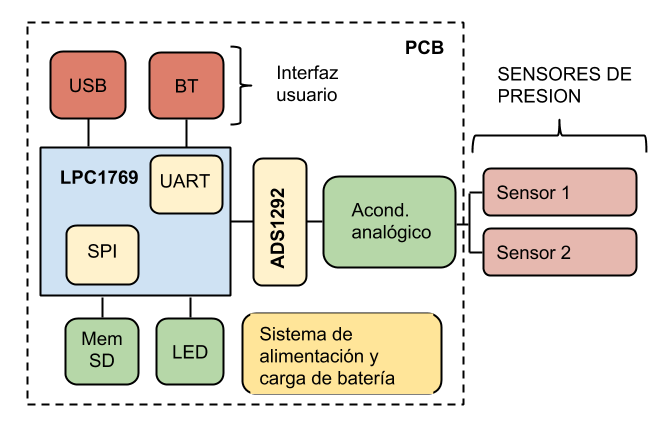
\includegraphics[width=\textwidth]{./Figures/diag_bloques.png}
	\caption{Diagrama en bloques del equipo.}
	\label{fig:diag_bloques}
\end{figure}

Para este proyecto se utilizaron en forma intensiva la gran mayoría de los contenidos y herramientas vistas durante el Curso de Especialización CESE. Se utilizaron técnicas de Gestión de Proyectos, documentación manual y automática del trabajo, sistema de versionado de software y hardware. En cuanto a lo técnico se emplearon conocimientos específicos sobre arquitectura del microcontrolador, modelos de programación, sistema operativo de tiempo real freeRTOS, protocolos de comunicación (BLE, SPI, USB, y de alto nivel), testing unitarios, etc.


\section{Motivación y Aplicaciones del equipo}

Para comprender de una forma más clara la necesidad y aplicaciones del equipo aquí presentado es imprescindible realizar una breve introducción teórica. El rol de la medición ambulatoria de presión arterial (MAPA) 24 hs braquial para predecir riesgo cardiovascular y mortalidad es ampliamente aceptado. Se sabe que la variabilidad de la presión arterial y su pulsatilidad son el resultado de una compleja interacción entre el corazón y la red vascular. En particular, y para la evaluación de las características biomecánicas de la red arterial, se utiliza la velocidad de onda de pulso (VOP) como indicador indirecto de rigidez arterial. Así como la MAPA braquial ha impulsado el desarrollo de dispositivos de registro y análisis cada vez más sofisticados, la posibilidad de realizar un registro ambulatorio de VOP genera nuevos campos de investigación, así como la necesidad de que existan nuevos dispositivos. 

Existen otros metodos de estimacion de la MAPA, pero se generan numerosas controversias debido a la complejidad matemática de las estimaciones y al uso de modelos matemáticos  arteriales unificados que suponen ser válidos para todos los pacientes. 
La presión arterial humana es responde a una curva que tiene un pico y un valle, y una forma de onda característica. De esta curva pueden calcularse toda una serie de parámetros que modelizan el arbol arterial. Sin embargo, el método más utilizado en la medicina clínica para estimar la presión arterial, el método oscilométrico, solo toma dos valores característicos de esta curva, el máximo y el mínimo, denominados \textbf{presion sistólica} y \textbf{presión diastólica}. Sin intentar profundizar en la técnica, el método oscilométrico consiste en inflar una almohadilla sobre el brazo del paciente a una presión que se supone mayor a lo normal en la población, de manera de obstruir por completo la circulación de la arteria a medir, colocando el sensor del estetoscopio bajo entre el brazo y la almohadilla. Luego se desinfla el manguito a una velocidad constante, y se mide en el manómetro la diferencia entre la presión arterial y de la almohadilla. Mientras se desinfla por encima del máximo de la curva de presión, la aguja del manómetro baja a ritmo constante. El operador de la medición, idealmente el personal de salud, visualiza en el manómetro el valor de presión para el cual la aguja hace un rebote. Este valor es la \textbf{presion sistólica}. La almohadilla sigue desinflándose, hasta un valor que ya no puede medirse diferencia contra la presión atmosférica. El último rebote de la aguja que se visualiza antes que se pierda la medición corresponde al mínimo, es decir \textbf{presión diastólica}. Esto puede visualizarse en la figura \ref{fig:presion}. Este método es de gran utilidad para la medicina clínica hace cientos de años, sin embargo, tiene la contrapartida de que se pierde el detalle de la forma de onda de la curva de presión, lo cual es solo posible apreciar utilizando un sistema de adquisición contínuo con una tasa de muestreo adecuada.


\begin{figure}[!htbp]
	\centering
	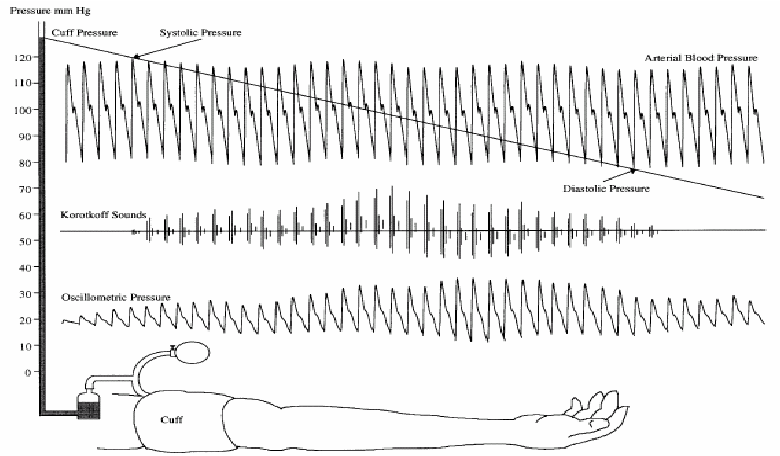
\includegraphics[width=\textwidth]{./Figures/presion.png}
	\caption{Curva de inflado del manguito de método del MAPA más utilizado vs presión real.\\ Presión diferencial medida y ruidos detectados.}
	\label{fig:presion}
\end{figure}


En este contexto, el estudio ambulatorio de la VOP en animales grandes podría brindar nuevas oportunidades para validar diferentes algoritmos de cálculo. La adquisición invasiva de señales de presión en dos sitios alejados del sistema arterial y a una distancia conocida, permite mejorar el conocimiento actual sobre la VOP en distintas condiciones del animal.


Las experiencias realizadas con este equipo permitirán profundizar la investigación sobre la medición indirecta de presión ambulatoria a partir de la medición de VOP y las técnicas para su cálculo. La aplicación de esta técnica para medición de presión ambulatoria permitirá desarrollar a futuro equipos ambulatorios que puedan medir de manera continua la presión de un paciente, con más información, mejor resolución y más comodidad al no tener un manguito inflable.

Las experiencias de medición de VOP se realizan sobre animales grandes concientes, como ovejas o cerdos. Estos animales se encuentran previamente instrumentados con sensores de presión intraarteriales en forma crónica y tienen un prolongado período de adaptación a la vida en un corral de un laboratorio de investigación y al trato con los veterinarios. En la figura \ref{fig:oveja} puede verse una fotografía de una oveja durante una experiencia real con un equipamiento antiguo. La correcta adaptación del animal a la vida en el corral del laboratorio es muy importante porque la medición de la presión arterial se ve severamente afectada por la comodidad y bienestar del animal. Por ejemplo, algunas de las líneas de investigación estudian justamente la diferencia de los valores medios de presión entre el período de vigilia y de sueño. Este tipo de experiencias sobre un animal en estado de alerta se hace totalmente imposible.


\begin{figure}[!htbp]
	\centering
	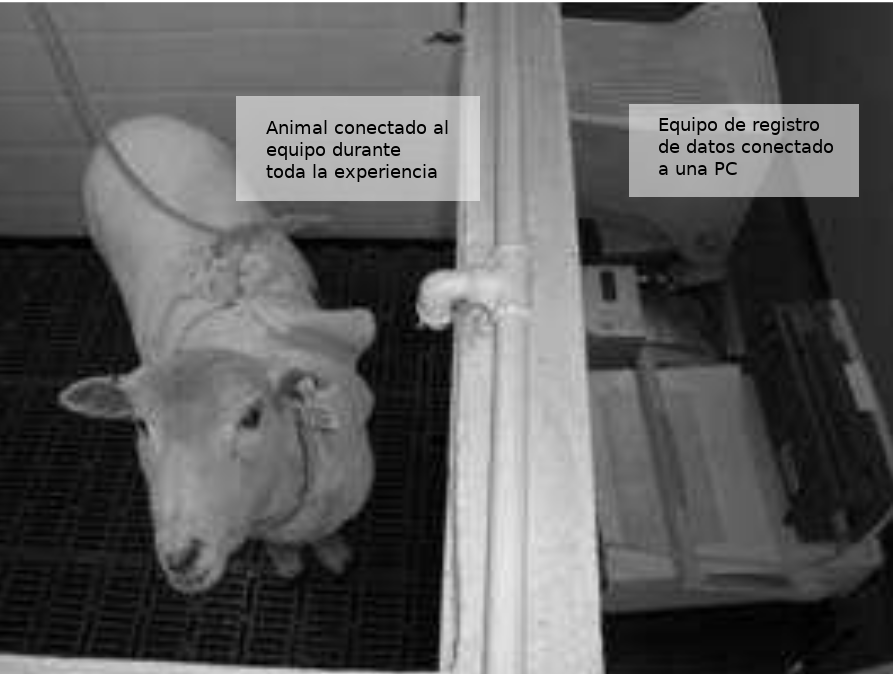
\includegraphics[width=\textwidth]{./Figures/oveja.png}
	\caption{Oveja instrumentada con un equipamiento antiguo con interfaz cableada.}
	\label{fig:oveja}
\end{figure}

El equipamiento de medición debe ir sobre el animal para evitar que existan cables que limiten el movimiento y dificulten la vida diaria del mismo. Además, luego de un período de adaptación, el equipo debe ser imperceptible para el animal. Esto se logra con un tamaño reducido, un sistema de carga cómoda, como una pequeña mochila, bajo peso, ausencia de ruido, etc. Durante toda la experiencia de medición, el equipo debe estar sobre el animal, y, dentro de lo posible, solo debe acercarse personal de veterinaria para tareas de higiene y alimentación, que son personas el animal ya conoce. El operador del equipo debería solamente acercarse al animal para la instalación del equipo, y para retirarlo al finalizar la experiencia. El resto del tiempo, el operador debe tener una interacción mínima con el animal.


\section{Objetivos y alcance}

El proyecto incluyó el desarrollo completo de un dispositivo de medición y adquisición de dos sensores de presión intraarteriales para ser utilizado en animales grandes, junto con su documentación técnica y manual de usuario. 

El equipo digitaliza señales analogicas provenientes de dos sensores de presión intrarterial del tipo strain-gauge y almacena las señales por períodos prolongados de alrededor de 24 hs. Estas señales adquiridas se guardan en una memoria de tipo flash (memoria SD), y pueden descargarse a una PC a través de una interfaz USB. Desde la PC se accede a los archivos guardados como un medio de almacenamiento masivo, y se pueden visualizar en cualquier software que permita procesar un archivo de tipo ".csv".

Previo a cada experiencia, el operador configura el equipo desde una terminal Bluetooth, como una tablet o una PC, a través de un protocolo de comunicación muy sencillo que se desarrolló para este proyecto. A través de esta interfaz se configuran parámetros como la frecuencia de muestreo, la cantidad de canales a usar, ganancia del amplificador programable, seteo de hora y fecha, y finalmente se da inicio a la medición. 

Las señales además se pueden visualizar en tiempo real para realizar algún eventual ajuste sobre el animal instrumentado antes de comenzar la experiencia. Este software de visualización no se incluye entre los alcances del proyecto, por lo que se utiliza solamente una interfaz en desarrollo a modo de prueba. 

El equipo se diseñó para ser portátil, alimentado por batería, con una autonomía aproximada de 24 horas. A la vez, se hizo énfasis en lograr un bajo peso que no moleste al animal durante la experiencia. La interfaz de carga es a través de la misma conexión USB.

El desarrollo del proyecto no incluye la fabricación del gabinete final ni del soporte para ser llevado por el animal. Tampoco se incluye el software de la terminal de configuración, solamente una versión beta para pruebas.
%----------------------------------------------------------------------------------------






